% !TEX spellcheck = en_US
%=================================================================================
\chapter{Controller Design Objectives}
%=================================================================================
The motivation of control in \gls{WT} is to optimize the energy production, avoid overspeed or other constraints and reduce structural loads \cite{SchlipfLecture}.
In order to manage the above named requirements there are different control tools used.
They are organized in an hierarchical order \cite{WindEnergyHandbook}:
\begin{enumerate} 
	\item safety system
	\item supervisory control
	\item \gls{CLC}
\end{enumerate} 
During the project of the \gls{shakti} turbine the focus was on the development of the \gls{CLC}.
%=================================================================================
\section{Closed-Loop Control (Soni)} \label{Advanced controller}
Figure \ref{fig:Closed-loop Wind Turbine Control} illustrates the \gls{CLC} system of a wind turbine.
The main control subject is the rotational speed of the turbine.
To obtain the desired behavior two different controllers are used, the pitch controller and the torque controller.

\begin{figure}[h]
	\centering
	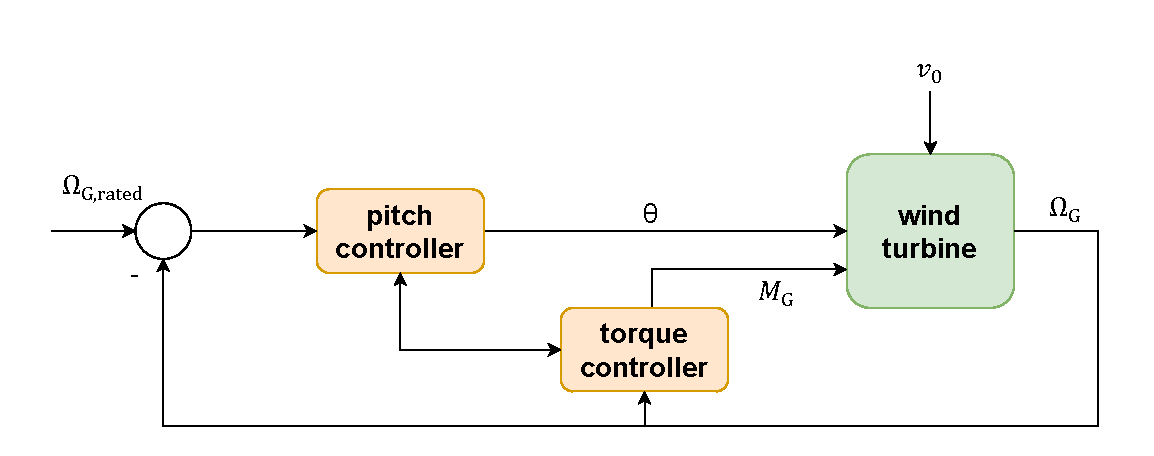
\includegraphics[width=\textwidth]{Figures/Control_loop}
	\caption{Closed-loop wind turbine control scheme}
	\label{fig:Closed-loop Wind Turbine Control}
\end{figure}

The torque controller optimizes power production below rated wind speed and maintain rated power above rated wind speed by adjusting generator torque (\gls{symb:M_G}) based on generator speed (\gls{symb:Omega_G}).
The torque controller uses a PI-controller with anti-windup to regulate the generator torque based on the difference between the actual and reference generator speed.
\\
\\
Above rated wind speed, the pitch controller maintains the rated generator speed (\gls{symb:Omega_G_rated}) by adjusting the blade pitch angle (\gls{symb:theta}), which ensures the rated power is maintained.
With increasing wind speed, the pitch angle increases to reduce the power coefficient (\gls{symb:cp}).
Once the wind speed reaches the rated value, the generator torque is maintained at its rated value.
The control is categorized into different regions, as detailed in section \ref{control regions}.
%=================================================================================
\section{Control Regions (Soni)} \label{control regions}

Wind turbine operations are segmented into three primary and two transition regions based on varying wind speed. These regions are explained in detail below and illustrated in Figure \ref{fig:control regions}.

\begin{figure}[h]
	\centering
	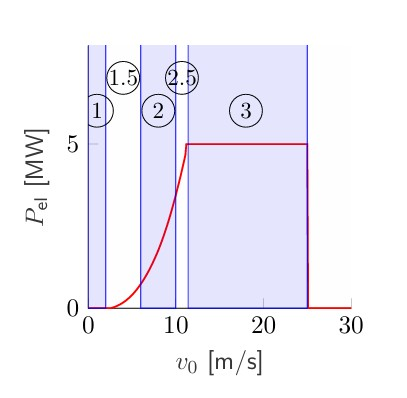
\includegraphics[width=0.5\textwidth]{Figures/Figure_2.jpg}
	\caption{Wind turbine control regions \cite{SchlipfLecture}}
	\label{fig:control regions} 
\end{figure}

\textbf{Control Region 1:} The wind speed is below the cut-in wind speed (\gls{symb:v_in}). 
The turbine does not generate any power.
There is no pitch activity.
\\
\\
\textbf{Control Region 1.5:} This is a transition to Region 2.
The wind speed is sufficient to accelerate rotor and increase the generator torque.
The goal is to quickly reach Region 2.
There is no pitch activity.
\\
\\
\textbf{Control Region 2:} Wind speeds are above the cut-in speed (\gls{symb:v_in}) but below the rated wind speed (\gls{symb:v_rated}). 
The primary objective is to maximize energy yield.
To achieve this, the power coefficient (\gls{symb:cp_opt}) is kept at its optimum. 
There is no pitch activity.
The control system ensures that the turbine maintains these optimal conditions by regulating the rotational speed through the torque controller.
In this region, the generator torque is adjusted based on rotor speed, as shown in Equation \ref{equation:MG}.

\begin{equation}
	M_{\textnormal{G}} = \frac{1}{2} \rho R^5 \frac{C_{\textnormal{P,opt}}}{{\lambda_{\textnormal{opt}}^3 r_{\textnormal{GB}}^3}} \Omega_{\textnormal{G}}^2
	\label{equation:MG}
\end{equation}

\begin{equation}
	M_{\textnormal{G}} = k\Omega_{\textnormal{G}}^2
	\label{equation:MG_2}
\end{equation}

\textbf{Control Region 2.5:} This is a transition to Region 3.
The rotational speed and the torque are raised until they reach the rated values. 
The goal is to quickly and smoothly reach Region 3.
There is no pitch activity.

\textbf{Control Region 3:} 
In this region, wind speeds have reached the rated wind speed.
The control goal is to maintain rated power and generator speed as well as reduce structural loads.
The pitch controller actively adjusts the blade pitch angle to regulate the speed and keep the power within the turbines rated conditions.
%=================================================================================
\section{Advanced Generator Torque Controller (Soni)} \label{Torque controller}
Generator torque is one of the two main control inputs for a wind turbine.
The performance of an advanced generator torque controller offers significant improvements and greater flexibility compared to a baseline torque controller.
The primary goal of the advanced torque controller is to reach the optimal power curve earlier and to maintain it for a longer duration compared to the baseline controller.
Additionally, the dynamics in Regions 1.5 and 2.5 are tunable, allowing for more precise control.
\\
\\
Goals of the advanced torque controller:
\begin{itemize}
	\item Achieve the optimal power curve earlier and maintain it for a longer period.
	\item Enable tunable dynamics in Regions 1.5 and 2.5.
	\item Interaction with PI-pitch controller to reduce loads and increase energy yield.
\end{itemize}

\begin{figure}[htbp]
	\centering
	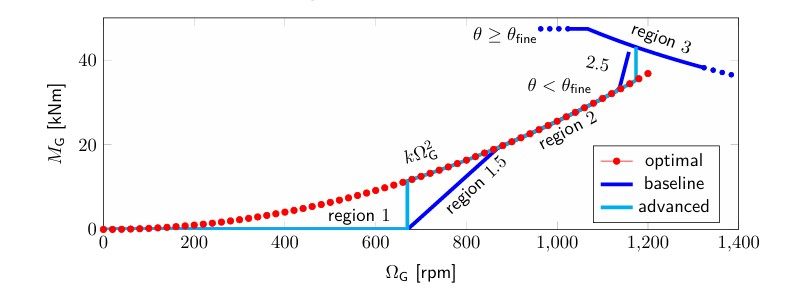
\includegraphics[width=\textwidth]{Figures/Figure_3.jpg}
	\caption{Wind turbine control regions \cite{SchlipfLecture}} 
	\label{WT control region}
\end{figure}

Strategy for the Advanced Torque Controller:

\textbf{Region 1.5:} Lowest generator speed $\Omega_{\textnormal{G,1.5}}$ set to avoid the 3P frequency interacting with the tower's eigenfrequency.

\textbf{Region 2:} The controller aims to maximize energy yield while ensuring the turbine operates efficiently.

\textbf{Region 2.5:} Generator speed $\Omega_{G,2.5}$ = $\Omega_{G,rated}$.
Switch from $\Omega_{\textnormal{G,1.5}}$ to $\Omega_{\textnormal{G,2.5}}$ if the measured generator speed \gls{symb:Omega_G} exceeds 

\begin{equation}
	\Omega_{\textnormal{G,R2switch}} = \frac{1}{2} (\Omega_{\textnormal{G,1.5}} + \Omega_{\textnormal{G,2.5}})
	\label{equation:Omega_Region_2.5}
\end{equation}

Torque Limits: 

The generator torque limits are determined by the measured generator speed \gls{symb:Omega_G} and incorporate Anti-Windup mechanisms.

\begin{itemize}
	
	\item if \gls{symb:Omega_G} < $\Omega_{\textnormal{G,R2switch}}$:
	
	\begin{equation}
		M_{\textnormal{G,lb}} = 0
		\label{equation:MG,lb}
	\end{equation}
	\begin{equation}
		M_{\textnormal{G,ub}} = k \Omega_{\textnormal{G}}^2
		\label{equation:MG,ub}
	\end{equation}
	
	\item if\gls{symb:Omega_G} > $\Omega_{\textnormal{G,R2switch}}$:
	
	\begin{equation}
		M_{\textnormal{G,lb}} = k \Omega_{\textnormal{G}}^2
		\label{equation:MG,lb,2}
	\end{equation}
	
	\begin{equation} 
		M_{\textnormal{G,ub}} = \min\left(M_{\textnormal{G,{rated}}}\frac{\Omega_{\textnormal{G,{rated}}}}{\Omega_{\textnormal{G}}}, M_{\textnormal{G,max}}\right)
		\label{equation:MG,ub,2}
	\end{equation}
	
\end{itemize}

\textbf{Region 3:} Adjusted limits for the generator torque based on the generator speed.

The design parameters for the PI controller are derived similar to exercise 3 of \cite{SchlipfLecture}.

\section{Collective Pitch Controller (CPC) (Julius)}
% !TEX spellcheck = en_US
% Collective Pitch Controller
%=================================================================================
Collective pitch control (CPC) adjusts the pitch for all 3 blades similarly.
The pitch control behavior has a high impact on the structural loads therefor on the life time of the wind turbine and thus on costs.
CPC can be implemented with a standard PI-Controller.
Main task of the CPC is to make the rotor area more permeable for the wind in order to reduce the power coefficient.
This is done by pitching the rotor blades in a less advantageous aerodynamic position.
With increasing wind speed the power output increases as well as the loads.
In order to keep the loads within an acceptable limit the power output of the wind turbine must be limited.

The pitch controller is only active in region 3, when the wind speed is above the rated wind speed as described in figure \ref{fig:control regions}.
In region 3 the pitch controller maintains rated speed and the generator torque controller rated torque.




\section{Tower Damper (Felix)}
% !TEX spellcheck = en_US
% Tower Damper
%=================================================================================
This section describes the function and the implementation of a pitch angle based \gls{td}. 
The design follows the description in \cite{WindEnergyHandbook} similar as the workflow in the exercise of the corresponding lecture \cite{SchlipfLecture}. 
The tower dynamics are modeled as in \cite{WindEnergyHandbook} (eq: 8.12 and 8.13). 
Here referred to as \ref{eq:TowerDynamics} and \ref{eq:TowerDamper}.
\begin{equation}
	M\ddot{x} + D\dot{x} + Kx = F + \Delta F
	\label{eq:TowerDynamics}
\end{equation}
\begin{equation}
	\begin{aligned}
		\Delta F = \frac{\partial F}{\partial \theta}\Delta\theta = -D_{\text{TD}}\dot{x}\\
		\Delta\theta = \frac{-D_{\text{TD}}}{\partial F/\partial \theta}\dot{x}
	\end{aligned}
	\label{eq:TowerDamper}
\end{equation}
As described by \ref{eq:TowerDynamics} the dynamics of the tower in fore-aft direction are lightly damped if $D$ is small and the force $\Delta F$ which is the additional thrust force resulting of a pitch action is equal to zero. The force $F$ is damped by the relative wind speed $v_{\text{rel}} = v_0 - \dot{x}$ and therefore $F = F(\Omega, \theta, v_{\text{rel}})$ \cite{SchlipfLecture}. To damp the tower top speed $\dot{x}$ even further \cite{WindEnergyHandbook} proposes an update of the pitch angle with $\Delta\theta$. This will damp the tower motion further as described in \ref{eq:TowerDamper}. This leads to a reduction of the tower bottom bending moment. Nevertheless this comes at a cost of higher pitch activity and the damping is only available in control region 3. 
%The static tower top deflection over the regions are shown in section \ref{steady states}. This is helpful to see when the damper is active and what can be damped.

The implementation and test of the damper is done in Matlab and Simulink.
As in the lecture \cite{SchlipfLecture} and corresponding exercise the tower top acceleration $\ddot{x}$ is used because it is a quantity that is measurable in reality as well.
What is also taken into account is the existence of a real pitch actuator. This means that the pitch update $\Delta\theta$ can not be applied instantaneously because of the time constant of the pitch actuator.
To address this phenomena there are 2 methods tested. 
First a direct integration \ref{eq:TDintegration}: 
\begin{equation}
	\dot{x}(t) = \int\ddot{x}(t) \text{d}t
	\label{eq:TDintegration}
\end{equation} 
And second a phase shift of \SI{90}{\degree} of the acceleration signal by a Lag-Compensator. The transfer function in the frequency domain is shown in \ref{eq:LagCompensator}. Where the input in the frequency domain is $\ddot{X}(s)$ and the output is $\dot{X}(s)$. 
\begin{equation}
	\frac{\ddot{X}(s)}{\dot{X}(s)} = \frac{s + z}{s + p}
	\label{eq:LagCompensator}
\end{equation} 
\begin{equation}
	\dot{x}(t) = \ddot{x}(t) - \int p\dot{x}(t) - z\ddot{x}(t) \text{d}t
	\label{eq:xddTimeDomain}
\end{equation} 

% explain analytical why this should work better?

The implementation in Simulink (Figure \ref{fig:TDoverview}) is first following the approach in the exercise \cite{SchlipfLecture}.

\begin{figure}[tbh]
	\centering	
	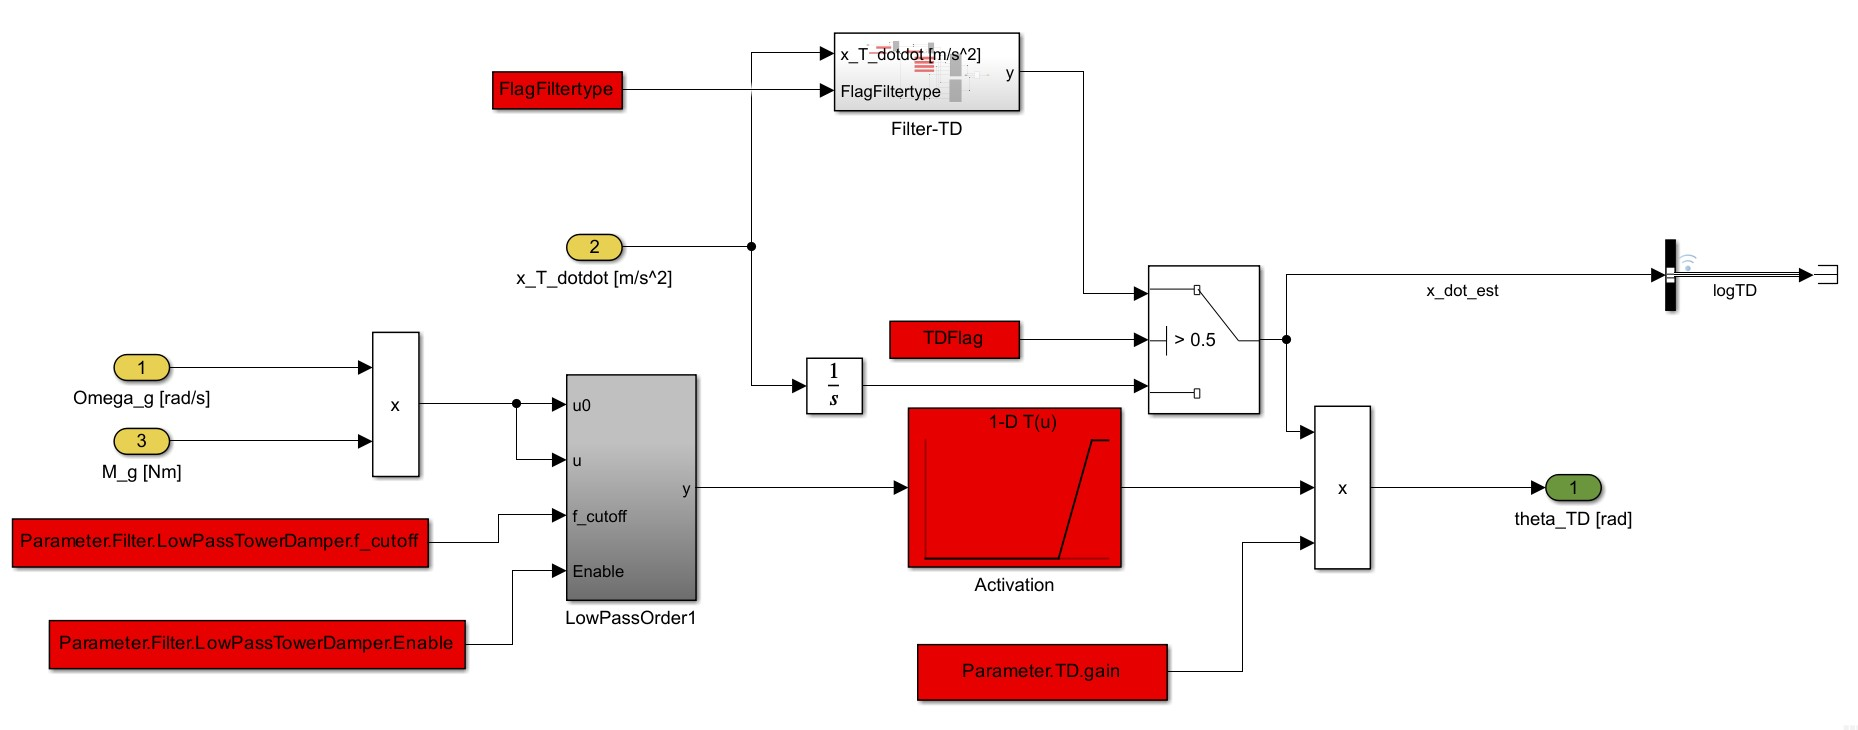
\includegraphics[width=12cm]{Figures/TDoverview}
	\caption{Tower Damper in Simulink model}
	\label{fig:TDoverview}
\end{figure} 

The input \textit{Omega\_g} is already a low pass filtered quantity and the blade passing frequency (3P) is notched out. As shown in Figure \ref{fig:TDoverview} to activate the \gls{td} the generator power is used. The \textit{LowPassOrder1} is used to reduce the switching frequency of the TD to ensure that it is not switched on and off if the \gls{WT} is operating near rated conditions. In the activation the gain is slowly ramped up from $\SI{0}{\%}$ to $\SI{100}{\%}$ over a power range from $\SI{80}{\%}$ of the rated power to $\SI{100}{\%}$.
For higher power values the gain stays at \SI{100}{\%}.

In the first method, here named integrator, the tower top acceleration signal is integrated.
The signal is than multiplied with the damping gain \textit{Parameter.TD.gain} and the activation signal as shown in Figure \ref{fig:TDoverview}.
The resulting quantity is the pitch offset mentioned in \ref{eq:TowerDamper}.
This offset $\Delta\theta$ is added to the pitch angle control value of the \gls{cpc} and this sum is the new input for the SLOW-model. In this first ideal method no pitch actuator is considered.

\begin{figure}[h]
	\centering	
	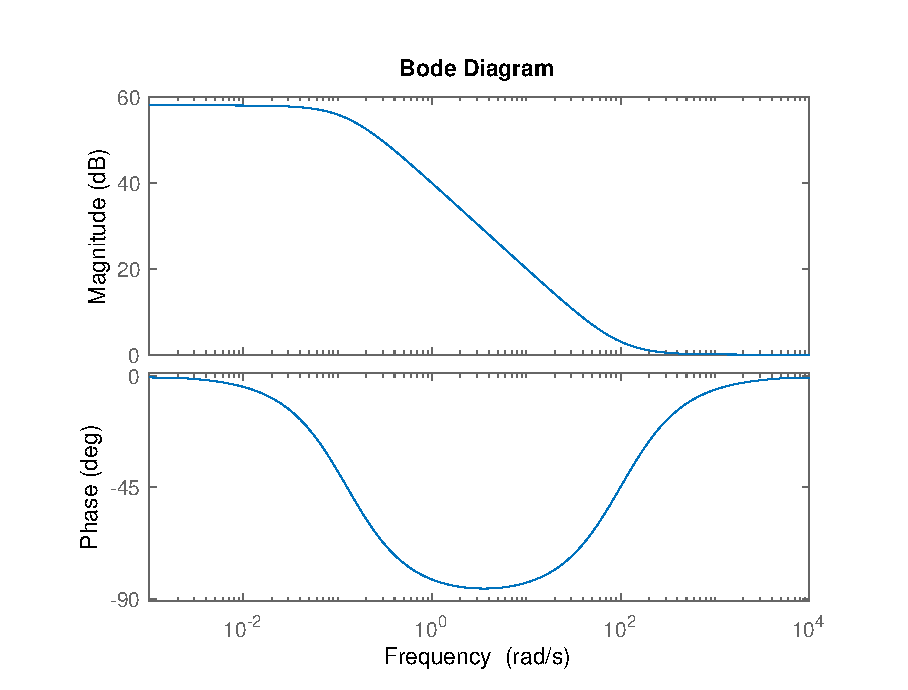
\includegraphics[width=12cm]{Figures/BodeLagCompensator.eps}
	\caption{Bode plot of the Lag-Compensator with tower eigenfrequency (black)}
	\label{fig:BodeLag}
\end{figure}

The second method, here named Lag-Compensator, isolates the tower eigenfrequency by passing the acceleration signal first through a low pass filter and than a high pass filter. The cutoff frequency of both filters is the eigenfrequency of the tower. Now the signal contains mainly the isolated eigenfrequency of the tower with which the tower is oscillating in the fore-aft direction. To phase shift the signal a Lag-Compensator is used. 


As shown in Figure \ref{fig:BodeLag} the frequency is phase shifted by nearly \SI{37}{\degree} and the magnitude is increasing by $\SI{23}{dB}$. This leads with an included pitch actuator that behaves like a PT2-Filter to an overall system shift of \SI{90}{\degree} and a magnitude increase of $\SI{16.5}{dB}$ see Figure \ref{fig:SystemBode}. The higher magnitude is adjusted by a different gain value.

\begin{figure}[h]
	\centering	
	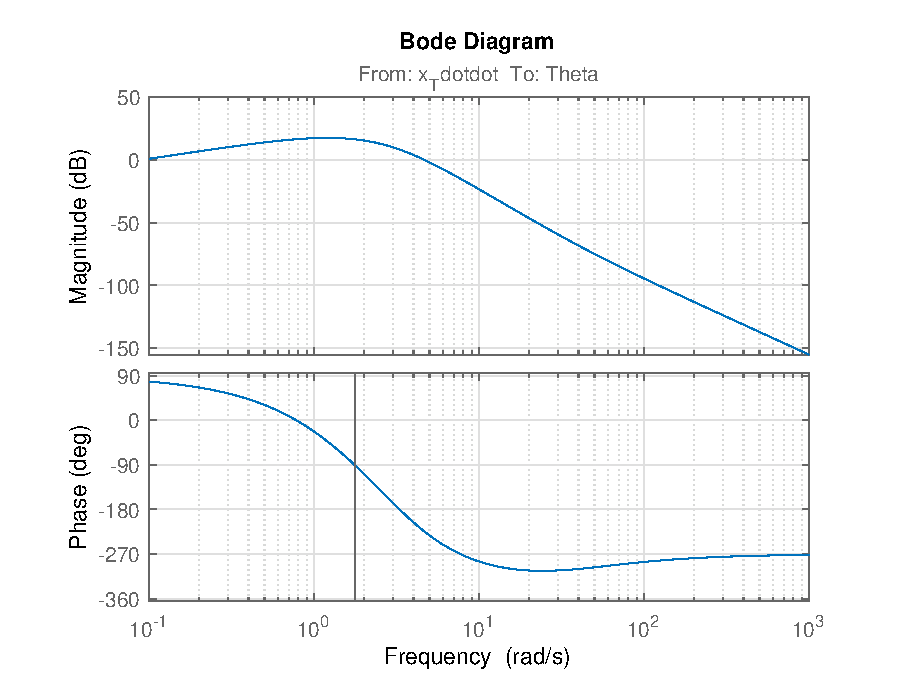
\includegraphics[width=12cm]{Figures/BodeSystem.eps}
	\caption{Bode plot of the Pitch-Actuator and Filter-Chain with tower eigenfrequency (black)}
	\label{fig:SystemBode}
\end{figure} 


The design is tested with a wind step from $v_0 = \SI{20}{m/s}$ to $v_1 = \SI{21}{m/s}$. The results are shown in Figure \ref{fig:TDWindStep}.

\begin{figure}[h]
	\centering	
	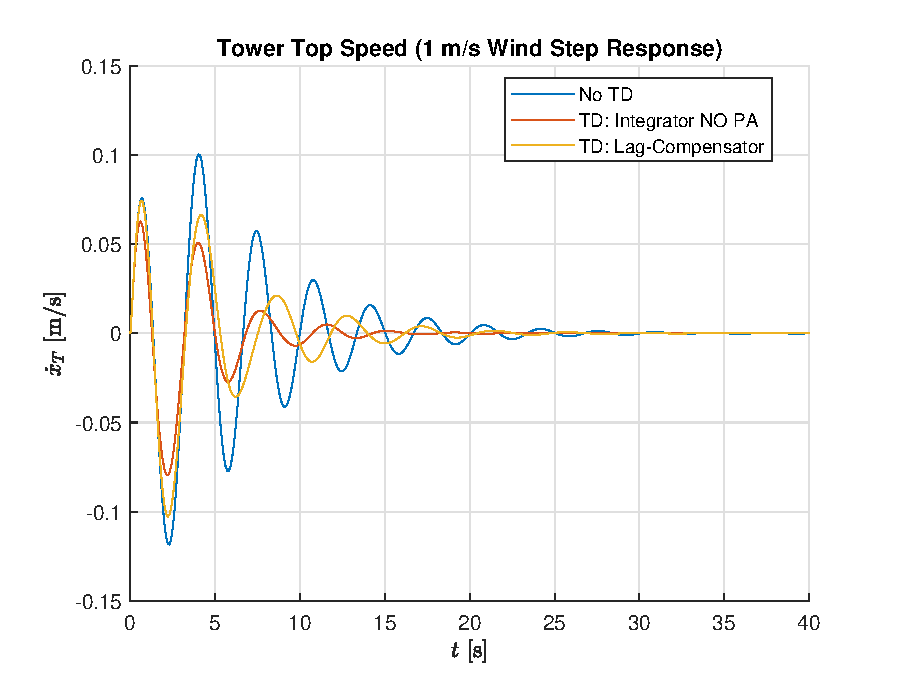
\includegraphics[width=12cm]{Figures/WindStep.eps}
	\caption{Tower-Top-Speed}
	\label{fig:TDWindStep}
\end{figure}

As shown in Figure \ref{fig:TDWindStep} the result is not matching the design and expectations above. 
The tower top speed is not in phase with the integrator method. It is to expect, that the implementation is containing an error.
To debug the system the filter and the integrator method are disturbed by a $\cos$-signal with the eigenfrequency of the tower as shown in Figure \ref{fig:Debug}. 
The two methods are not perfectly aligned. 
The difference at the beginning is not the issue but that the signals are not converting into the same is causing the issue. 
First fine tuning iterations of the Lag-Compensator does not lead to a successful result. 
This issue remains unsolved by the end of the project end requires a deeper investigation. 
 
\begin{figure}[h]
	\centering	
	\includegraphics[width=12cm]{Figures/Debugging.eps}
	\caption{Debugging of the \gls{td} with Lag-Compensator}
	\label{fig:Debug}
\end{figure}
  
The expected result with the filter result is, that the loads at the eigenfrequency of the tower are reduced the same way as they are with an integrator.
But due to the fact that the filter is considering the signal delay by the pitch actuator the loads around the eigenfrequency are not increased as with a pure integrator.    
